% (c) 2015 Daniele Zambelli daniele.zambelli@gmail.com
% (c) 2016 Andrea Sellaroli andrea.sellaroli@istruzione.it

\input{\folder calc_combinatorio_grafici.tex}

\chapter{Calcolo combinatorio}

Uno dei problemi principali che dovremo saper risolvere per calcolare la 
probabilità di un evento, è quello di \emph{contare} in quanti modi può 
presentarsi un certo evento. 
Alcuni esempi tipici che studieremo in questo capitolo saranno:
\begin{enumerate}[nosep]
\item quante combinazioni diverse posso ottenere nel lancio di un dado e una 
moneta;
\item in quanti modi diversi posso ordinare gli oggetti di un insieme;
\item quanti sono gli anagrammi di una parola;
\item in quanti modi diversi può essere costituito il podio di una gara;
\item quante sono le combinazioni di una cassaforte;
\item in quanti modi diversi posso estrarre un sottoinsieme di elementi da un 
insieme;
\item in quanti modi diversi posso ordinare una coppa di gelato.
\end{enumerate}

% quante password di 6 caratteri posso ottenere? Quanti anagrammi della parola 
% "MATEMATICA" posso fare? Quante sono le possibili colonne del totocalcio?

\section{Prodotto cartesiano}
\label{sec:calc_combinatorio_prodotto}

Partiamo da un esempio sufficientemente semplice
\begin{esempio}
Quante configurazioni diverse ottengo dal lancio di una dado e di una moneta?
Nel lancio della moneta ho 2 possibilità, per ognuna di queste il dado 
offre altre 6 possibilità. 
Possiamo rappresentare la situazione con un grafo ad albero:

\medskip
\affiancati{.48}{.48}{
Prima la moneta poi il dado: 
% Se inizio lanciando la moneta ho 2 possibilità. \\
% per ognuna di queste ho 6 possibilità con il lancio del dado: 
\begin{center} \scalebox{.7}{\monetadadoalbero} \end{center}
}{
Prima il dado poi la moneta: 
% Se inizio lanciando il dado ho 6 possibilità. \\
% per ognuna di queste ho 2 possibilità con il lancio della moneta: 
\begin{center} \scalebox{.7}{\dadomonetaalbero} \end{center}
}

\medskip
Quello che ottengo è il \emph{prodotto cartesiano} dei due insiemi di 
eventi possibili:
\begin{align*}
M \times D = 
\begin{Bmatrix} 
\punto{T}{1},~ \punto{T}{2},~ \punto{T}{3},~
\punto{T}{4},~ \punto{T}{5},~ \punto{T}{6}, \\
\punto{C}{1},~ \punto{C}{2},~ \punto{C}{3}, 
\punto{C}{4},~ \punto{C}{5},~ \punto{C}{6} 
\end{Bmatrix}
\end{align*}
Cambiare l'ordine dei due eventi (prima il dado poi la moneta) corrisponde, 
nel prodotto cartesiano, a scambiare gli elementi di ogni coppia ordinata. 
Le diverse configurazioni possibili sono 12.
% \begin{align*}
% M \times D = 
% \begin{Bmatrix} 
% \punto{1}{T},~ \punto{2}{T},~ \punto{3}{T},~
% \punto{4}{T},~ \punto{5}{T},~ \punto{6}{T}, \\
% \punto{1}{C},~ \punto{2}{C},~ \punto{3}{C}, 
% \punto{4}{C},~ \punto{5}{C},~ \punto{6}{C} 
% \end{Bmatrix}
% \end{align*}
Possiamo rappresentare la situazione anche con un grafo cartesiano:
\medskip

\affiancati{.48}{.48}{
Prima la moneta poi il dado: 
\begin{center} \scalebox{.7}{\monetadadocart} \end{center}
}{
Prima il dado poi la moneta: 
\begin{center} \scalebox{.7}{\dadomonetacart} \end{center}
}
\end{esempio}

\begin{newoss}{}{}
È abbastanza evidente che il numero di eventi possibili non cambia se lancio 
prima il dado o prima la moneta.
\end{newoss}

Il numero di elementi del prodotto cartesiano è uguale al prodotto del 
numero di elementi di ogni insieme.

\begin{newdef}{}{}
Il numero di eventi possibili dati dalla combinazione di eventi semplici 
indipendenti è il prodotto delle possibilità degli eventi semplici.
\end{newdef}

\begin{esempio}
In un armadio ci sono 6 magliette, 4 paia di pantaloni, 2 cappelli e 3 paia 
di scarpe. 
In quanti modi diversi è possibile vestirsi?

% Costruiamo quattro caselle che corrispondono ai quattro capi di abbigliamento 
% del problema. La prima casella, ad esempio, è quella relativa alle magliette 
% che possono essere scelte in 6 modi diversi; la seconda è quella dei 
% pantaloni, che possono essere scelti in 4 modi diversi.
% \begin{center}
% \begin{tabular}{cccc}
% \fbox{6} & \fbox{4} & \fbox{2} & \fbox{3}\\
% \end{tabular}
% \end{center}
In questo caso risulta piuttosto lungo e complicato realizzare un grafo che 
riporti tutte le possibilità o scrivere tutte quadruple possibili, ma il 
numero di elementi del prodotto cartesiano si ottiene facilmente:
\[\text{numero elementi}\tonda{M \times P \times C \times S} = 
  6 \cdot 4 \cdot 2 \cdot 3 = 144\]
\end{esempio}

\section{Permutazioni}
\label{sec:calc_combinatorio_permutazioni}

Capita spesso di dover scegliere degli elementi da un insieme finito e di 
doverli ordinare in una sequenza. 
Anche in questo caso partiamo da un esempio semplice.
\begin{esempio}
Tre studenti, Alice, Barbara e Carlo, devono decidere in che ordine 
presentarsi ad un'interrogazione programmata.
In quanti modi possibili possono organizzarsi?

Proviamo a visualizzare la cosa. Il primo studente può essere scelto 
all'interno dell'insieme \(\{\)Alice, Barbara, Carlo\(\}\), che contiene 3 
elementi. 
Possiamo rappresentarlo con un diagramma ad albero:

\vspace{-6pt}
\begin{center}
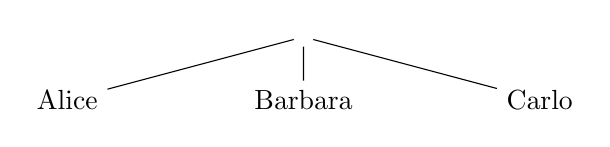
\begin{tikzpicture}[level distance=8mm,
  level 1/.style={sibling distance=3cm},
  level 2/.style={sibling distance=1.5cm}]
  \node {}
    child {node {Alice}}
    child {node {Barbara}}
    child {node {Carlo}};
\end{tikzpicture}
\end{center}
% \vspace{-6pt}
Il secondo interrogato dovrà essere scelto tra i due non già interrogati:

% \vspace{-12pt}
\begin{center}
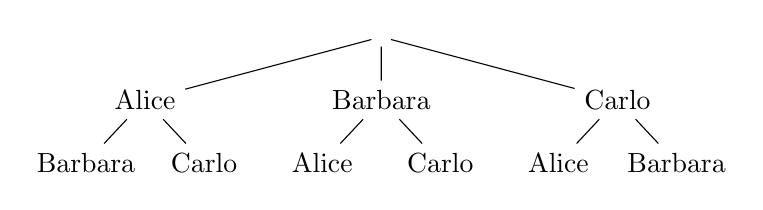
\begin{tikzpicture}[level distance=8mm,
  level 1/.style={sibling distance=3cm},
  level 2/.style={sibling distance=1.5cm}]
  \node {}
    child {node {Alice}
      child {node {Barbara}}
      child {node {Carlo}}
    }
    child {node {Barbara}
      child {node {Alice}}
      child {node {Carlo}}
    }
    child {node {Carlo}
      child {node {Alice}}
      child {node {Barbara}}
    };
\end{tikzpicture}
\end{center}
La scelta del terzo studente è obbligata e l'albero completo si presenta 
così:

% \vspace{-12pt}
\begin{center}
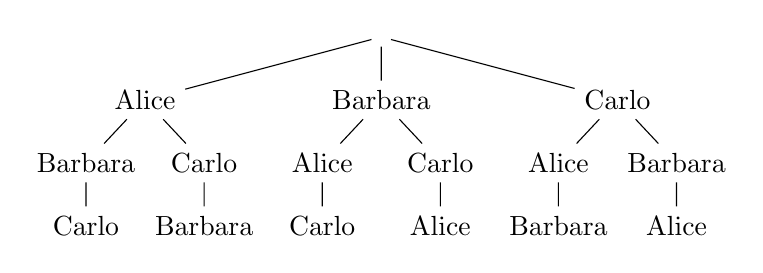
\begin{tikzpicture}[level distance=8mm,
  level 1/.style={sibling distance=3cm},
  level 2/.style={sibling distance=1.5cm}]
  \node {}
    child {node {Alice}
      child {node {Barbara} child {node {Carlo}}}
      child {node {Carlo} child {node {Barbara}}}
    }
    child {node {Barbara}
      child {node {Alice} child {node {Carlo}}}
      child {node {Carlo} child {node {Alice}}}
    }
    child {node {Carlo}
      child {node {Alice} child {node {Barbara}}}
      child {node {Barbara} child {node {Alice}}}
    };
\end{tikzpicture}
\end{center}

Ognuno dei possibili ordinamenti è rappresentato in un percorso che va 
dalla radice dell'albero fino ad una foglia (nodo terminale). 
In totale i possibili ordinamenti sono quindi 6:

\begin{center}
\begin{tabular}{c|c|c}
Alice, Barbara, Carlo & Barbara, Alice, Carlo & Carlo, Alice,Barbara\\
\hline
Alice, Carlo, Barbara & Barbara, Carlo,Alice & Carlo, Barbara,Alice\\
\end{tabular}
\end{center}

\vspace{.2cm}
Un altro modo di vedere la cosa è il seguente. 
Immaginiamo di avere tre scatole vuote che rappresentano le tre posizioni 
in cui possono essere interrogati i tre studenti.
\begin{center}
\begin{tabular}{ccc}
\fbox{\phantom{3}} & \fbox{\phantom{2}} & \fbox{\phantom{1}}\\
\end{tabular}
\end{center}
Il primo studente può essere scelto in 3 modi diversi. Il secondo, essendo 
già stato scelto il primo, potrà essere effettuata tra due possibilità. 
L'ultimo è obbligato essendo rimasto solo.
\begin{center}
\begin{tabular}{ccc}
\fbox{3} & \fbox{2} & \fbox{1}\\
\end{tabular}
\end{center}
Possiamo quindi determinare il numero di ordinamenti possibili moltiplicando 
il numero di scelte possibili ad ogni livello: 
\(6 = 3 \cdot 2 \cdot 1\) modi diversi. 
\end{esempio}

La generalizzazione di questa idea prende il nome di \emph{principio di 
moltiplicazione}. 
Se una scelta può essere fatta in \(n_1\) modi diversi, e per ciascuno di 
questi modi una seconda scelta può essere fatta in \(n_2\) modi diversi, 
e per ognuno dei modi in cui sono fatte le due prime scelte una terza 
scelta può essere fatta in \(n_3\) modi diversi, e così via per \(k\) 
scelte, allora il numero totale di scelte è 
\(n_1 \cdot n_2 \cdot n_3 \cdot ... \cdot n_k\).
Analizzeremo nel seguito diversi casi che si presentano con una certa 
frequenza e che possono essere risolti utilizzando il principio di 
moltiplicazione.

Abbiamo visto che per ordinare 3 studenti sono possibili 6 modi distinti. E se 
gli studenti fossero 10? 
Il primo studente lo posso scegliere in 10 modi diversi, il secondo solo in 9 
modi diversi, visto che il primo è già stato scelto, il terzo in 8 modi e 
così via.

\begin{center}
\begin{tabular}{cccccccccc}
\fbox{10} & \fbox{9} & \fbox{8} & \fbox{7} & \fbox{6} & \fbox{5} & \fbox{4} & 
\fbox{3} & \fbox{2} & \fbox{1}\\
\end{tabular}
\end{center}

Applicando il principio di moltiplicazione il numero degli ordinamenti 
possibili è quindi 
\(10\cdot 9\cdot 8\cdot 7\cdot 6\cdot 5\cdot 4\cdot 3\cdot 2\cdot 1 = 
  3\,628\,800\). 

Questo prodotto ha per fattori tutti i numeri naturali da 1 a 10. È 
un'importante operazione matematica che prende il nome di \emph{fattoriale}. 
\begin{newdef}{}{}
Il \emph{fattoriale} di un numero naturale \(n\), indicato con \(n!\), è il 
prodotto dei numeri interi positivi minori o uguali ad \(n\):
\[0! = 1; \quad 1! = 1 \quad n! = n \cdot \tonda{n-1}!\]
ovvero: 
\[n! = n \cdot (n-1) \cdot (n-2) \cdot \dots \cdot 3 \cdot 2 \cdot 1\] 
\end{newdef}
I primi fattoriali sono dunque:
\begin{center}
\begin{tabular}{lll}
\(0! = 1\) & \(1! = 1\) & \(2! = 2 \cdot 1 = 2\)\\
\(3! = 3 \cdot 2 = 6\) & 
\(4! = 4 \cdot 6 = 24\) & 
\(5! = 5 \cdot 24 = 120\)\\
\(6! = 6 \cdot 120 = 720\) & 
\(7! = 7 \cdot 720 = 5040\) & 
\(8! = 8 \cdot 5040 = 40\,320\)\\
\(9! = 9 \cdot 40\,320 = 362\,880\) & 
\(10! = 10 \cdot 362\,880 = 3\,628\,800\) & 
\(11! = 11 \cdot 3\,628\,800 = 39\,916\,800\)
\end{tabular}
\end{center}

Per la soluzione più rapida degli esercizi può essere utile imparare a 
memoria i primi fattoriali (fino a \(8!\)).

A questo punto possiamo generalizzare al caso di un insieme formato da \(n\) 
elementi. 

\begin{newdef}{}{}
Le \emph{permutazioni} di \(n\) elementi sono tutti i possibili ordinamenti 
che si possono effettuare con \(n\) oggetti. 
Il numero delle permutazioni è:
\[P_n = n!\]
\end{newdef}

Un esempio comune di permutazioni è dato dagli anagrammi.
% \begin{exrig}
\begin{esempio}
Quanti sono i possibili anagrammi, anche senza senso, della parola 
``VERONA''?

Gli elementi da permutare sono 6 e tutti diversi tra loro, 
quindi tutti i possibili anagrammi sono \(P_6 = 6!= 720\).
\end{esempio}
% \end{exrig}



% \begin{osservazione}
%  Nell'esempio che abbiamo appena visto sarebbe considerata una grande 
% ingiustizia se il nome di uno studente comparisse due volte nell'elenco. In 
% questo caso di dice che tale problema è \emph{senza ripetizioni}. In molte 
% situazioni però è normale che gli elementi possano essere ripetuti, basta 
% pensare che per formare un numero di telefono non c'è alcun problema se 
% alcune 
% cifre compaiono più volte. Nei prossimi paragrafi analizzeremo tutte le 
% casistiche che si possono presentare.
% \end{osservazione}

\section{Permutazioni con ripetizione}
\label{sec:calc_combinatorio_con_ripetizione}

Quando parliamo di animali, di piante o, in generale, di oggetti, ognuno ha 
una propria individualità, è composto da atomi diversi, e non è lo stesso 
mettere prima uno o prima una altro anche se si assomigliano.
Ma quando abbiamo a che fare con simboli, la situazione cambia:
``AA'' è lo stesso di ``AA'' anche se ho scambiato la prima con la seonda 
``A''.

Nell'esempio precedente abbiamo potuto usare il \emph{principio della 
moltiplicazione} perché le lettere che formano la parola VERONA sono tutte 
diverse. Nel caso in cui una lettera venga ripetuta più volte la situazione è 
più complessa.
Proviamo ad analizzare tutti i possibili anagrammi della parola MAMMA: in 
questo caso compaiono 3 volte la lettera M e 2 volte le lettere A. Per calcolare 
il numero di possibili anagrammi ragioniamo nel modo seguente. Mettiamo un 
indice alle lettere uguali per distinguerle:
\[M_1 A_1 M_2 M_3 A_2\]
Se calcolo tutte le possibili permutazioni risulta \(5! = 120\). 
Tuttavia le due permutazioni 
\(M_1 M_2 M_3 A_1 A_2\) e \(M_1 M_2 M_3 A_2 A_1\) 
rappresentano la stessa parola ``MMMAA''. 
Le 120 permutazioni che si ottengono se le lettere sono 
distinguibili va quindi diviso per le possibili permutazioni della lettera 
``M'' che sono \(3!=6\) e della lettera ``A'' che sono \(2!\). 

In definitiva tutti gli anagrammi della parola MAMMA sono:
\(\dfrac{5!}{2!\cdot 3!}=10\).

\begin{definizione}
Le \emph{permutazioni con ripetizione} di \(n\) elementi di cui 
\(k_1\) uguali tra loro, \(k_2\) uguali tra loro e distinti dai precedenti, 
\dots , \(k_p\) uguali tra loro e distinti dai precedenti, sono:
\[P_n^{\tonda{k_1;~k_2;~\dots;~k_p}} = 
  \dfrac{n!}{k_1!\cdot k_2! \cdot \text{\dots} \cdot k_p!}\]
\end{definizione}

\begin{esempio}
Quanti sono i possibili anagrammi della parola MATEMATICA?
Le lettere che formano la parola ``MATEMATICA'' sono 10. 
La lettera ``A'' è ripetuta 3 volte, le lettere ``M'' e ``T'' sono ripetute 
2 volte. I possibili anagrammi sono quindi:
\[P_{10}^{\tonda{3;~2;~2}}=\dfrac{10!}{3!\cdot 2! \cdot 2!} =
\dfrac{3\,628\,800}{6 \cdot 2 \cdot 2} = 151\,200\]
\end{esempio}


\section{Disposizioni}
\label{sec:calc_combinatorio_disposizioni}
Nelle permutazioni il numero di elementi ed il numero di posti è uguale. 
In alcune situazioni può capitare che il numero dei posti sia inferiore al 
numero di elementi. 

Partiamo da un esempio:
\begin{esempio}
Quante sono le parole di tre lettere, anche 
senza significato, che si possono formare usando le 26 lettere dell'alfabeto 
italiano\footnote{~Per chi ha frequentato le scuole elementari può risultare 
strano che le lettere dell'alfabeto italiano siano 26, ma basta aprire un 
qualunque dizionario della lingua italiana per averne la prova.} senza che ci 
siano lettere ripetute? 

Come per i casi precedenti, la prima lettera può essere scelta in 26 modi 
diversi, la seconda solo in 25 e la terza in 24 modi:
\begin{center}
\begin{tabular}{ccc}
\fbox{26} & \fbox{25} & \fbox{24}\\
\end{tabular}
\end{center}

Il risultato è che le possibili parole di 3 lettere in modo che non compaiano 
lettere ripetute è \(26 \cdot 25 \cdot 24 = 15\,600\).

Si può riscrivere questo calcolo usando il fattoriale in una forma che ci 
sarà utile nella definizione: 
\[26 \cdot 25 \cdot 24 =
26 \cdot 25 \cdot 24 \cdot \dfrac{23!}{23!} = 
\dfrac{26 \cdot 25 \cdot 24 \cdot 23!}{23!} = 
\dfrac{26!}{23!}=\dfrac{26!}{(26-3)!}\]
\end{esempio}

\begin{newdef}{}{}
Le \emph{disposizioni} di \(n\) elementi in \(k\) posti, con \(n\geq k\), sono tutte 
le scelte ordinate di \(k\) elementi presi tra gli \(n\) disponibili. 
Il numero delle disposizioni è
\[D_{n,~k} = 
\underbrace{n\cdot (n-1) \cdot (n-2) \cdot \text{\dots} \cdot (n-k+1)}
_{\text{k elementi}} =
\dfrac{n!}{(n-k)!}\]
\end{newdef}

\begin{esempio}
In un gruppo di 19 studenti, in quanti modi possono scelti 4 studenti per 
essere interrogati?
In questo caso abbiamo \(19\) elementi per \(4\) posti, quindi:
\[D_{19,~4} = 19\cdot 18 \cdot 17 \cdot 16 = \dfrac{19!}{(19-4)!}= 
\dfrac{19!}{15!} = 93024\]

\end{esempio}

\section{Disposizioni con ripetizione}
\label{sec:calc_combinatoio_disposizioni_con_ripetizione}

Quando abbiamo a che fare con simboli, ogni elemento di un insieme può 
essere scelto più di una volta.
Ad esempio, nel caso delle parole di tre lettere potrei scegliere la 
stessa lettera più volte.
In tal caso non vale più il ragionamento precedente, infatti dopo aver scelto 
una lettera questa rimane ancora disponibile per la scelta successiva.
\begin{center}
\begin{tabular}{ccc}
\fbox{26} & \fbox{26} & \fbox{26}\\
\end{tabular}
\end{center}
La formula finale non farà uso del fattoriale, ma sarà semplicemente una 
potenza.

\begin{definizione}
Le \emph{disposizioni con ripetizione} di \(n\) elementi, in \(k\) posti sono 
tutte le scelte ordinate (anche ripetute) di \(k\) elementi tra gli \(n\) 
disponibili.
Il numero di tali disposizioni è dato da:
\[D_{n,~k}' = n^k\]
\end{definizione}

\begin{esempio}
Devo scegliere una password di 5 cifre per il mio nuovo smartphone.
Quante diverse password è possibile creare? Notiamo che ogni cifra può essere 
scelta casualmente tra le 10 disponibili 
\(\{0;~1;~2;~3;~4;~5;~6;~7;~8;~9\}\), 
e è possibile anche ripetere una cifra più volte (infatti
ha perfettamente senso scegliere come password, per esempio, il codice 
232425). Quindi:
\[D_{10,~5}' = 10^5 = 100\,000 \quad \tonda{\text{da} \quad 00000 \sstext{a} 
99999}\]
\end{esempio}

\section{Combinazioni}
\label{sec:calc_combinatorio_combinazioni}
Esaminiamo i seguenti problemi, all'apparenza molto simili:
\begin{itemize}[noitemsep]
\item Da un insieme di 10 studenti ne seleziono 4 da interrogare in 4 giorni distinti.
\item Da un insieme di 10 studenti ne seleziono 4 da interrogare lo stesso giorno.
\end{itemize}
In entrambi i problemi abbiamo \(n=10\) elementi da distribuirsi in \(k=4\) posti. 
Nel primo caso, tuttavia, l'ordine è importante, mentre nel secondo 
è indifferente in che sequenza vengono scelti.
La soluzione del primo caso è una \emph{disposizione}, come visto nel paragrafo 
precedente:
\[D_{10,~4} = \dfrac{10!}{(10-4)!}=\dfrac{10!}{6!}=5040\]

Se gli studenti vengono interrogati contemporaneamente non ha alcuna importanza 
in che ordine vengono scelti. 
Tra le \(5040\) possibilità precedenti ce ne sono ovviamente molte di uguali. Se 
indichiamo con A,B,C e D ognuna dei seguenti ordini è conteggiato nei \(5040\):
\begin{center}
\begin{tabular}{cccccc}
\(A B C D\) & \(A B D C\) & \(A C B D\) & \(A C D B\) & \(A D B C \) & 
\(A D C B\)\\
\(B A C D\) & \(B A D C\) & \(B C A D\) & \(B C D A\) & \(B D A C \) & 
\(B D C A\)\\
\(C A B D\) & \(C A D B\) & \(C B A D\) & \(C B D A\) & \(C D A B \) & 
\(C D B A\)\\
\(D A C B\) & \(D A B C\) & \(D C A B\) & \(D C B A\) & \(D B A C \) & 
\(D B C A\)\\
\end{tabular}
\end{center}
In totale fanno \(24\) ordini possibili che è il numero di permutazioni di 4 
elementi, infatti \(4!=24\). Questa situazione si ripete uguale per ogni 
possibile scelta dei quattro elementi tra i 10. Se non siamo interessati 
all'ordine quindi possiamo dividere il numero di disposizioni di 10 
elementi in 4 posti per il numero di permutazioni di 4 elementi.

\[C_{10,~4} = \dfrac{D_{10,~4}}{4!} = \dfrac{10!}{4! \tonda{10 -4}!}=
\dfrac{10!}{4!~6!} = 
\dfrac{10 \cdot 9 \cdot 8 \cdot 7 \cdot 6!}{4 \cdot 3 \cdot 2 \cdot 6!} = 
210\]
Generalizzando otteniamo:
\begin{newdef}{}{}
Le \emph{combinazioni} di \(n\) elementi di classe \(k\) sono ognuna delle scelte 
di \(k\) elementi tra gli \(n\) senza che conti l'ordine in cui sono scelti. Il 
numero delle combinazioni è
\[C_{n,~k} =  \dfrac{n!}{k!(n-k)!}\]
\end{newdef}

\begin{esempio}
Quante sono le possibili cinquine che si possono fare nella tombola (90 numeri)?

Si tratta delle combinazioni di 90 elementi in 5 posti (infatti non è 
importante l'ordine in cui i numeri vengono estratti per fare cinquina). Le 
possibilità sono quindi:
\[C_{90,~5} =  \dfrac{90!}{5!(90-5)!}=43 949 268\]
\end{esempio}

Vista la grande importanza che rivestono, il numero delle combinazioni si 
indica con un simbolo specifico, detto \emph{coefficiente binomiale}.

\begin{newdef}{}{}
Il \emph{coefficiente binomiale} è definito come 
\[\binom{n}{k}=\dfrac{n!}{k!(n-k)!}\]
\end{newdef}

\section{Combinazioni con ripetizione}
\label{sec:calc_combinatoio_combinazioni_con_ripetizione}

Come nelle disposizioni, anche nelle combinazioni in certe situazioni gli 
elementi possono essere ripetuti \\[4pt]
Tralasciamo in questo caso di ricavare la formula e ci limitiamo soltanto 
ad esibirla.

\begin{newdef}{}{}
Le \emph{combinazioni con ripetizione} di \(n\) elementi di classe \(k\) 
sono ognuna delle scelte di \(k\) elementi, anche ripetuti, tra gli \(n\), 
senza che conti l'ordine in cui sono scelti. 
Il numero delle combinazioni è
\[C_{n,k}' =  C_{n+k-1,k} = \binom{n+k-1}{k} = \dfrac{(n+k-1)!}{k!(n-1)!}\]
\end{newdef}

\begin{esempio}
In quanti modi diversi possono essere scelte delle coppe di gelato da 5 
gusti, potendo scegliere anche più palline dello stesso gusto, sapendo che 
la gelateria dispone di 8 gusti?

Poiché in una coppa di gelato non conta l'ordine in cui vengono messe le 
palline, si tratta certamente di combinazioni. 
Avendo poi la possibilità di scegliere più palline uguali, 
il numero delle combinazioni con ripetizione è:
\[C_{8,~5}' = C_{\tonda{8+5-1},~5} = C_{12,~5} = \binom{12}{5} = 
\frac{12!}{5!~7!} =
\frac{12 \cdot 11 \cdot 10 \cdot 9 \cdot 8 \cdot \cancel{7!}}{5 \cdot 4 \cdot 
3\cdot 2\cdot 1 \cdot \cancel{7!}}=792\]
\end{esempio}

\section{Compendio}
\label{sec:calc_combinatoio_compendio}

Può succedere che difronte ad un problema ci si trovi in imbarazzo nel capire 
se si tratta di Prodotto, di Disposizioni, di Combinazioni, \dots

Di seguito riporto una procedura che si può seguire per facilitare la 
decodifica del problema.

\begin{procedura} Per individuare il tipo di calcolo combinatorio relativo a 
un problema:
\begin{enumerate} %[nosep]
\item 
Abbiamo più insiemi e dobbiamo scegliere un solo elemento per insieme?

Allora si tratta di \emph{Prodotto Cartesiano}: \hfill 
\(PC = a \cdot b \cdot c \cdot \text{\dots}\).

\item 
Abbiamo un solo insieme, dobbiamo utilizzare tutti i suoi elementi e è 
importante l'ordine?

Allora si tratta di \emph{Permutazioni}.
\begin{enumerate}[nosep]
\item Gli elementi non possono essere ripetuti?

Allora si tratta di \emph{Permutazioni Semplici}: \hfill 
\(P_n = n!\).
\item Gli elementi possono essere ripetuti?

Allora si tratta di \emph{Permutazioni con Ripetizione}: \\ 
\phantom{0}\hfill
\(P_n^{\tonda{k_1;~k_2;~\dots;~k_p}} = 
  \dfrac{n!}{k_1!\cdot k_2! \cdot \text{\dots} \cdot k_p!}\).
\end{enumerate}

\item 
Abbiamo un solo insieme, ci interessano solo un certo numero dei suoi 
elementi e è importante l'ordine?

Allora si tratta di \emph{Disposizioni}.
\begin{enumerate}[nosep]
\item Gli elementi non possono essere ripetuti?

Allora si tratta di \emph{Disposizioni Semplici}: \\ 
\phantom{0}\hfill
\(D_{n,~k} = n\cdot (n-1) \cdot \text{\dots} \cdot (n-k+1) = 
\dfrac{n!}{(n-k)!}\).
\item Gli elementi possono essere ripetuti?

Allora si tratta di \emph{Disposizioni con Ripetizione}: \hfill 
\(D_{n,~k}' = n^k\).
\end{enumerate}

\item 
Abbiamo un solo insieme, ci interessano solo alcuni dei suoi elementi 
e non è importante l'ordine?

Allora si tratta di \emph{Combinazioni}.
\begin{enumerate}[nosep]
\item Gli elementi non possono essere ripetuti?

Allora si tratta di \emph{Combinazioni Semplici}: \hfill 
\(\displaystyle C_{n,~k} = \binom{n}{k} = \dfrac{n!}{k! \tonda{n-k}!}\).
\item Gli elementi possono essere ripetuti?

Allora si tratta di \emph{Combinazioni con Ripetizione}: \\ 
\phantom{0}\hfill
\(\displaystyle C_{n,~k}' = \binom{n+k-1}{k} = 
                \dfrac{\tonda{n+k-1}!}{k! \tonda{n-1}!}\).
\end{enumerate}
\end{enumerate}
\end{procedura}

